\section{Application to consumer theory}
Constant Elasticity of Substitution (CES) functions have been applied extensively to Consumer Theory as seen in our literature review. There are two main reasons why the CES function is so popular in Consumer Theory literature. The first is that its flexibility allows several different relations between goods depending on the value of $\rho$; that is, it is easy to represent perfect compliments (Leontieff shaped utility), perfect substitutes (linear utility), and Cobb-Douglas preferences using the CES utility function. Hence, CES functions are a general case that don't impose too many restrictions on the type of preference the function represents.
\subsection{Characterization in terms of preferences}
The characters of CES function in terms of preference include but are not limit to the following.
\subsubsection{Constant elasticity of substitution}
The first particular characteristic of CES functions that is useful is its constant elasticity of substitution between two goods. That is,\\

$$e_{ij}\left( p,w\right) = - \dfrac{\partial\left[ x_{i}\left( p,w\right)/x_{j}\left( p,w\right) \right] }{\partial\left[ p_{i}/p_{j}\right]} \dfrac{p_{i}/p_{j}}{x_{i}\left( p,w\right)/x_{j}\left( p,w\right)}=\dfrac{1}{1-\sigma}$$

Intuitively, this tells us that the percent increase in relative consumption given a percent change in relative prices will be constant.
Other important characteristics of the CES function include consumers' taste for variety and when the CES function is concave. When we derive these important characteristics, we assume prices are strictly greater than zero, and that the utility function is continuous, differentiable, and locally nonsatiated.
\subsubsection{Taste for variety}
CES preferences imply a taste for variety. To show this, we use a simplified form of CES function and assume symmetry in prices and consumption. The prices of products are given as, $p_1 = \cdots = p_L = p$ and parameters in CES function are all given as unity, that is, $a_1 = \cdots = a_L = 1$. The number of products is given by $L$, so that an increase in $L$ represents the increase in product diversity.

The total expenditure can be represented as
\begin{equation}
I = Lpx.
\end{equation}

Consequently, the demand function can be simplified to,
\begin{equation}
x_{i} = x = \frac{w}{Lp}
\end{equation}

Hence, the indirect utility function can be simplified to,
\begin{equation}
\ln(u) = \ln w + \ln\left(L^{\frac{1-\sigma}{\sigma}}\right) +  \ln\left(p^{\frac{1-\sigma}{\sigma}}\right) \label{eq:variety1}
\end{equation}

Differentiating the indirect utility function \eqref{eq:variety1} gives,

\begin{equation}
\frac{du}{u}  = \left(\frac{1-\sigma}{\sigma}\right) \frac{dL}{L} + \left(\frac{1-\sigma}{\sigma}\right) \frac{dp}{p}
\end{equation}

For simpler notation, define $\hat{x} = \frac{dx}{x}, \hat{u} = \frac{du}{u},\hat{p} = \frac{dp}{p} \text{and } \hat{L} = \frac{dL}{L}$. Then,

\begin{equation}
\hat{u} = \left(\frac{1-\sigma}{\sigma}\right) \hat{L} + \left(\frac{1-\sigma}{\sigma}\right) \hat{p} \label{eq:diversity2}
\end{equation}

From \eqref{eq:diversity2}, we can see that utility increases as variety increases when $\sigma$ is less than 1, and $\sigma \neq 0$ which is in the parameter range for the CES utility function suggested in the earlier sections.
\subsubsection{Concavity of utility function}
Consider a CES utility function with constant returns:

\begin{equation}
u(x_{1},...,x_{n}) = \sum\limits_{l=1}^{L} a_{l} x_{l}^{\sigma}
\end{equation}
This function will be concave if $a_{l}\geq0$ for all $l$ and $\sigma\leq1$. We prove this by first showing that $u$ is quasi-concave. \\
A function is a quasi-concave function if it is a monotone increasing function of a concave function. So let's look for a simple function ``hidden inside'' of $u$.

We note that then
\begin{equation}
u(x)=g(x)^{\frac{1}{\sigma}}
\end{equation}
where
\begin{equation}
g(x)=\sum\limits_{l=1}^{n} a_{l} x_{l}^{\sigma}
\end{equation}

Suppose that $0<\sigma\leq1$. Then we see from Equation 2 that $u(x)$ is a monotone increasing function of $g(x)$. Now it is easy to verify if $0<\sigma\leq1$, then $g(x)$ is concave function, because its Hessian is simply a diagonal matrix with entries of the form:

\begin{equation}
a_{l}\sigma(1-\sigma)x_{l}^{\sigma-2}
\end{equation}

When $0<\sigma\leq1$, this term is non-positive. There $u(x) = g(x)^{\frac{1}{\sigma}}$ is a monotone decreasing fuction of $g(x)$. But if it is a monotone decreasing function of $g(x)$, it is a monotone increasing function of $-g(x)$. Now when $\sigma<0$, the Hessian matrix of $-g(x)$ is a diagonal matrix with entries of the form:

\begin{equation}
-a_{l}\sigma(\sigma-1)x_l^{\sigma-2}
\end{equation}

When $\sigma<0$, these terms are all non-positive and hence $-g$ is a concave function. Then $u(x)$ is a monotone increasing function of $-g(x)$, it must be that $u$ is quasiconcave.

We next show more that $u$ is a concave function. Because $u$ is quasi-concave function that is homogeneous of degree 1, $u$ must also be concave.

We now generalize this for CES functions that are homogeneous of type less than 1. When $u(x)$ is the constant returns to scale function defined, the CES functions that are of degree $k$ less than 1 take the form $u(x)^{k}$ where $0 < k < 1$. Now if we have a concave function $u: \mathbb{R}^{n} \rightarrow \mathbb{R}$, and an increasing concave function $g: \mathbb{R} \rightarrow \mathbb{R}$, then if we define the function $h: \mathbb{R}^n \rightarrow \mathbb{R}$ so that $h(x) = g(u(x))$, then $h$ must be a concave function.

\subsubsection{Completeness}
Preference that generated a CES utility function is complete.
$$\forall x_1, x_2 \in X^L, \quad u(x_1)\geq u(x_2) \quad or \quad u(x_1)\leq u(x_2)$$
$$\therefore x_1 \precsim x_2\quad or \quad x_1 \succsim x_2 $$
\subsubsection{Transitivity}
Preference that generated a CES utility function is transitive.
$$\forall x_1, x_2,x_3 \in X^L, \text{if} \hspace*{2mm} x_1 \succsim x_2 \hspace*{2mm} and \hspace*{2mm} x_2 \succsim x_3$$
$$\quad u(x_1)\geq u(x_2) \quad and \quad u(x_2)\geq u(x_3)$$
$$\therefore u(x_1)\geq u(x_3)$$
$$x_1 \succsim x_3$$
\subsubsection{Monotonicity}
Preference that generated a CES utility function is strongly monotone.
$$\forall x, y \in X^L, \text{if} \hspace*{2mm} x\geq y  \hspace*{2mm} \text{and} \hspace*{2mm} x\neq y$$
$$\text{then}  \hspace*{2mm} x_{i}>y_{i}  \hspace*{2mm}\text{for some} \hspace*{2mm} i  \hspace*{2mm} \text{and} \hspace*{2mm} x_j=y_j  \hspace*{2mm} \text{for}  \hspace*{2mm} j\neq i$$
Let $\Delta x_i = x_i-y_i$
\begin{align*}
u(x) &= \left(\sum_{l=1}^{L}a_lx_l^\sigma\right)^{\dfrac{1}{\sigma}}\\
     &= \left(\sum a_ix_i^\sigma+\sum a_jx_j^\sigma\right)^{\dfrac{1}{\sigma}}\\
     &= \left(\sum a_i(y_i+\Delta x_i)^\sigma+\sum a_jy_j^\sigma\right)^{\dfrac{1}{\sigma}}\\
     &>\left(\sum_{l=1}^{L}a_ly_l^\sigma \right)^{\dfrac{1}{\sigma}} = u(y)
\end{align*}
$$\therefore x\succ y$$
\subsubsection{Convexity}
Preference that generated a CES utility function is strictly convex.
$$\forall x, y,z \in X^L, \text{if} \hspace*{2mm} x\succsim z,  \hspace*{2mm} y\succsim z \hspace*{2mm} \text{and} \hspace*{2mm} x\neq y$$
Let $\alpha \in (0,1)$. $ x\succsim z$ and $y\succsim z$, so $u(x)\geq u(z)$ and $u(y)\geq u(z)$.
\vspace*{1mm}
$$u(\alpha x+(1-\alpha)y)  \hspace*{27mm}$$
\vspace*{-10mm}
\begin{align*}
&= \left(\sum_{l=1}^{L}a_l(\alpha x_l+(1-\alpha)y_l)^\sigma\right)^{\dfrac{1}{\sigma}} \\
& >  \left(\sum_{l=1}^{L}a_l\alpha x_l^\sigma+(1-\alpha)y_l^\sigma\right)^{\dfrac{1}{\sigma}}\\
&= \left(\alpha\sum_{l=1}^{L}a_l x_l^\sigma+(1-\alpha)\sum_{l=1}^{L}a_l y_l^\sigma\right)^{\dfrac{1}{\sigma}}\\
& > \alpha\left(\sum_{l=1}^{L}a_l x_l^\sigma\right)^{\dfrac{1}{\sigma}}+(1-\alpha)\left(\sum_{l=1}^{L}a_l y_l^\sigma\right)^{\dfrac{1}{\sigma}}\\
& \geq \alpha u(z)+(1-\alpha) u(z)\\
&=u(z)
\end{align*}
$$\therefore \alpha x+(1-\alpha)y \succ z$$
\subsubsection{Homotheticity}
Preference that generated a CES utility function is homothetic.
$$\forall x, y \in X^L, \text{if} \hspace*{2mm} x\sim y,  \hspace*{2mm} u(x)=u(y) $$
\begin{align*}
u(tx) =& \left(\sum_{l=1}^{L}a_ltx_l^\sigma\right)^{\dfrac{1}{\sigma}}\\
      =& t\left(\sum_{l=1}^{L}a_lx_l^\sigma\right)^{\dfrac{1}{\sigma}}\\
      =& tu(y)\\
      =&u(ty)
\end{align*}
$$\therefore tx\sim ty$$
\subsection{Constrained optimization}
We derive the demand function under a CES utility function. Our utility maximization problem is,
\begin{IEEEeqnarray}{l}
    \max u = \left( \sum_{l=1}^L a_l x_l^{\sigma} \right)^{\dfrac{1}{\sigma}} \\
    \qquad \text{s.t.} \nonumber \\
    \qquad \qquad \sum_{l=1}^L p_l x_l(p,w) \leq w \nonumber \\
    \qquad \qquad x_l \geq 0, \quad \forall l \in \{1, 2, \cdots, L\}
\end{IEEEeqnarray}
Lagrangian for this problem is,
\begin{IEEEeqnarray}{rCl}
    \mathcal{L} (x,\lambda) & = & \left( \sum_{l=1}^L a_l x_l^{\sigma} \right)^{\frac{1}{\sigma}} + \lambda\left(w - \sum_{l=1}^L p_l x_l\right) + \sum_{l=1}^L \mu_l x_l
\end{IEEEeqnarray}
First order conditions for this problem are,
\begin{IEEEeqnarray}{rCl}
    \frac{\partial \mathcal{L} \left( x, \lambda \right)}{\partial x_j} & = & \left( \sum_{l=1}^L a_l x_l^{\sigma} \right)^{\frac{1-\sigma}{\sigma}}+ a_j x_j^{\sigma-1} - \lambda p_j + \mu_j = 0 \label{eq:foc_j} \\
    \frac{\partial \mathcal{L} (x,\lambda)}{\partial x_k} & = & \left( \sum_{l=1}^L a_l x_l^{\sigma} \right)^{\frac{1-\sigma}{\sigma}} +a_k x_k^{\sigma-1} - \lambda p_k + \mu_k = 0 \label{eq:foc_k} \\
    && \sum_{l=1}^L p_l x_l(p,w) \leq w \nonumber \\
    && \mu_l x_l = 0 \nonumber \\
    && \mu_l \geq 0, x_l \geq 0, \lambda \geq 0 \quad \forall l \in \{1, 2, \cdots, L\} \nonumber
\end{IEEEeqnarray}
If we assume $x_j, x_k > 0$ for any $j$, $k$, and $\mu_j = \mu_k = 0$, then rearranging \eqref{eq:foc_j}, and \eqref{eq:foc_k} gives,
\begin{IEEEeqnarray}{rCl}
    \left( \sum_{l=1}^L a_l x_l^{\sigma} \right)^{\frac{1-\sigma}{\sigma}} \frac{1}{\lambda} & = & \left( \frac{p_j}{a_j} \right) x_l^{1-\sigma} \label{eq:foc_j2} \\
    \left( \sum_{l=1}^L a_l x_l^{\sigma} \right)^{\frac{1-\sigma}{\sigma}} \frac{1}{\lambda} & = & \left( \frac{p_k}{a_k} \right) x_k^{1-\sigma} \label{eq:foc_k2}
\end{IEEEeqnarray}
Equating the righthand side of \eqref{eq:foc_j2} and \eqref{eq:foc_k2} gives,
\begin{IEEEeqnarray}{l}
    x_j^{1-\sigma}\left(\frac{p_j}{a_j}\right) = x_k^{1-\sigma}\left(\frac{p_k}{a_k}\right) \nonumber \\
    \Rightarrow x_j = x_k \left( \frac{p_k}{a_k} \right)^{\frac{1}{1-\sigma}} \left( \frac{p_j}{a_j} \right)^{\frac{-1}{1-\sigma}} \label{eq:foc_comb}
\end{IEEEeqnarray}
Multiplying $p_j$ to both sides of equation \eqref{eq:foc_comb} and summing up over index $j$ gives,
\begin{IEEEeqnarray}{l}
    \sum_{j=1}^L p_j x_j = \sum_{j=1}^L p_j x_k \left( \frac{p_k}{a_k} \right)^{\frac{1}{1-\sigma}} \left( \frac{p_j}{a_j} \right)^{\frac{-1}{1-\sigma}} \nonumber \\
    \Rightarrow w = x_k \left( \frac{p_k}{a_k} \right)^{\frac{1}{1-\sigma}} \sum_{j=1}^L \left( \frac{p_j}{a_j} \right)^{\frac{-1}{1-\sigma}} \label{eq:foc_comb2}
\end{IEEEeqnarray}
Rearranging \eqref{eq:foc_comb2} gives the demand function for $x_k$, which is
\begin{IEEEeqnarray}{rCl}
    x_k & = & \frac{w\left(\frac{p_k}{a_k}\right)^{\frac{1}{\sigma-1}}}{\sum_{j=1}^L p_j \left( \frac{p_j}{a_j}\right)^{\frac{1}{\sigma-1}}} \label{eq:demand}
\end{IEEEeqnarray}

\subsection{Typical manipulations}
\subsubsection{Marginal Rate of Substitution}
The marginal utility for good $x_k$ is
$$MU(x_k) = \dfrac{\partial u(x)}{\partial x_k} = a_kx_k^{\sigma-1}\left(\sum_{l=1}^{L}a_lx_l^\sigma\right)^{\dfrac{1}{\sigma}-1}$$
$$MRS_{kj} = \dfrac{MU(x_k)}{MU(x_j)} = \dfrac{a_k}{a_j}\left( \dfrac{x_k}{x_j} \right)^{\sigma-1} $$
Notice here the marginal utility for good $x_k$ depends on all goods and their parameters. But the marginal rate of substitution for goods $x_k,x_k$ depends only themselves.
\subsubsection{Assumption of $a_l$}
Normally people assume that the sum of $a_l$  equals to one for convenience. Also under this assumption, $a_l$ provides us an insight for the expenditure share of good $x_l$ which we will discuss later.
$$\sum_{l=1}^{L}a_l = 1$$
\subsection{Interpretation in the context of consumption}
Let $p_{l}$ be the price of good $l$.
\subsubsection{Expenditure Share}
Expenditure Share of Good $x_l$:
\begin{equation}
	S_{l} = \dfrac{p_{l}\left(\dfrac{p_{l}}{a_{l}}\right)^{\frac{1}{ \sigma -1}}}{ \sum_{i=1}^L {p_{l}{\left(\dfrac{p_{i} }{a_{l}}\right)^{\frac{1}{ \sigma -1}}}}}
\end{equation}
The expenditure share responds to price change of any good. This also means that when the price of one good $x_l$ changes, the expenditure share of all goods will change.
\subsubsection{Changes of expenditure Share}
Change of the share with respect to price where $S_l = \dfrac{p_lx_l}{w}$:
\begin{equation}
	\frac{\partial{S_{l}}}{\partial{P_{l}}} <0
\end{equation}
When the price of good $x_l$increases, the expenditure share of that good decreases which means consumers switch to goods other than $x_l$

Change of the share with respect to wealth:
\begin{equation}
	\frac{\partial{S_{k}}}{\partial{w}} = 0
\end{equation}
The expenditure share of any good will not respond on wealth level changes.
\subsubsection{Indirect utility function}
Indirect Utility:
\begin{equation}
  	V= U\left(x\left(p_{1},...,p_{L},w\right)\right) = \frac{w}{ \left(\sum_{l=1}^La_{l}^{\frac{\-1}{\sigma-1}}p_{l}\right)^{\frac{\sigma-1}{ \sigma}}}
\end{equation}
Notice here the indirect utility is a homogeneous of degree one with respect to wealth level.
\subsubsection{Relative Demand}
Relative Demand:
\begin{equation}
	\frac{x_{k}}{x_{j}} = \dfrac{\left(\dfrac{p_{k}}{\alpha_{k}}\right)^{\frac{1}{ \sigma -1}}}{\left(\dfrac{ p_{j} }{\alpha_{j}}\right)^{\frac{1}{ \sigma -1}}} = \left(\dfrac{a_jp_{k}}{a_kp_{j}}\right)^{\dfrac{1}{ \sigma -1}} \label{eq:reldemand}
\end{equation}
The relative demand is important here for the reason that we have a constant elasticity of substitution only for the relative demand when there are more than two goods.
\subsubsection{Interpretation of $\sigma$}
$\sigma$ gives us an insight of the elasticity of substitution.
$$e_{ij} = \dfrac{1}{\sigma-1}$$
$$\sigma = \dfrac{e_{ij}+1}{e_{ij}}$$
A higher $\sigma$ means consumers are easily to substitute between goods. When $\sigma \to 1$, goods become perfectly substitutes. When $\sigma \to -\infty$, consumers are hard to substitute between goods which makes them have a Leontief utility function.
\subsubsection{Interpretation of $a$}
$a_l$ is called the share parameter, and we normally we have the assumption that $\sum_{l=1}a_{l}=1$. It also gives us an insight of the marginal utility. Let the marginal utility of good $x_k$ be $MU(x_K)$.
$$MU(x_k) = \dfrac{\partial u(x)}{\partial x_k} = a_kx_k^{\sigma-1}\left(\sum_{l=1}^{L}a_lx_l^\sigma\right)^{\frac{1}{\sigma}-1}$$
So here a larger $a_k$ implies that good $x_k$ has a larger marginal utility
\subsection{Special case of two goods}
The utility maximization problem an representative individual faces is as following, where $0 \neq \sigma \leq 1 $. Here we have goods $x$, $y$ and wealth level $w$. And the prices are denote as $p_x$ and $p_y$ respectively.
\begin{equation}
\begin{array}{rlclcl}
\displaystyle \max_{x,y} & \multicolumn{3}{l}{u(x)=(ax^\sigma+by^\sigma)^{\frac{1}{\sigma}}}\\
\textrm{s.t.} & w=p_{x}x+p_{y}y
\end{array}
\end{equation}

Setting up the Lagrangian
\begin{equation}
\mathcal{L}(x,y,\lambda)=(ax^\sigma+by^\sigma)^{\frac{1}{\sigma}}-\lambda(p_{x}x+p_{y}y-w)
\end{equation}
F.O.C.
\begin{equation}
\frac{\partial \mathcal{L}(x,y,\lambda)}{\partial x} =a(ax^\sigma+by^\sigma)^{\frac{1-\sigma}{\sigma}}x^{\sigma-1}-\lambda p_{x}=0
\end{equation}

\begin{equation}
\frac{\partial \mathcal{L}(x,y,\lambda)}{\partial y} =b(ax^\sigma+by^\sigma)^{\frac{1-\sigma}{\sigma}}b^{\sigma-1}-\lambda p_{y}=0
\end{equation}
\begin{equation}
\frac{\partial \mathcal{L}(x,y,\lambda)}{\partial \lambda} =-(p_{x}x+p_{y}y-w)=0
\end{equation}

Combining first and second equations above,
\begin{equation}
\frac{x}{y} =(\frac{bp_{x}}{ap_{y}})^{\dfrac{1}{\sigma-1}} \Rightarrow x= (\frac{bp_{x}}{ap_{y}})^{\frac{1}{\sigma-1}}y
\end{equation}
Plug this into the budget constraint equation
\begin{equation}
x=\frac{w(bp_{x})^{\frac{1}{\sigma-1}}}{b^{\frac{1}{\sigma-1}}p_{x}^{\frac{\sigma}{\sigma-1}}+a^{\frac{1}{\sigma-1}}p_{y}^{\frac{\sigma}{\sigma-1}}}
\end{equation}

\begin{equation}
y=\frac{w(ap_{y})^{\frac{1}{\sigma-1}}}{b^{\frac{1}{\sigma-1}}p_{x}^{\frac{\sigma}{\sigma-1}}+a^{\frac{1}{\sigma-1}}p_{y}^{\frac{\sigma}{\sigma-1}}}
\end{equation}
Therefore, the constant elasticity of substitution could be derived
\begin{equation}
\frac{x}{y}=(\frac{p_{x}}{p_{y}}\frac{b}{a})^{\frac{1}{\sigma-1}} \Rightarrow ln\frac{x}{y}=\frac{1}{\sigma-1}ln\frac{p_{x}}{p_{y}}+\frac{1}{\sigma-1}ln\frac{b}{a} \Rightarrow \frac{d ln\frac{x}{y} }{ d ln\frac{p_{x}}{p_{y}}}=\frac{1}{\sigma-1}
\end{equation}
The indirect utility function is

\begin{equation}
v(p_{x},p_{y},w)=\frac{w}{(a^{-\frac{1}{\sigma-1}}p_{x}^{\frac{\sigma}{\sigma-1}}+b^{-\frac{1}{\sigma-1}}p_{y}^{\frac{\sigma}{\sigma-1}})^{\frac{\sigma-1}{\sigma}}}
\end{equation}

The preference relationship represented by CES utility function is homothetic, the indifference curves have the same slope at $(x,y)$ and at $(tx,ty)$ for any $t > 0$. The indifference curves below are drawn based on the CES utility function $u(x,y)=(3x^{0.5}+4y^{0.5})^2$. We draw four indifference curves under utility level at 15, 18, 20 and 22.
\begin{center}
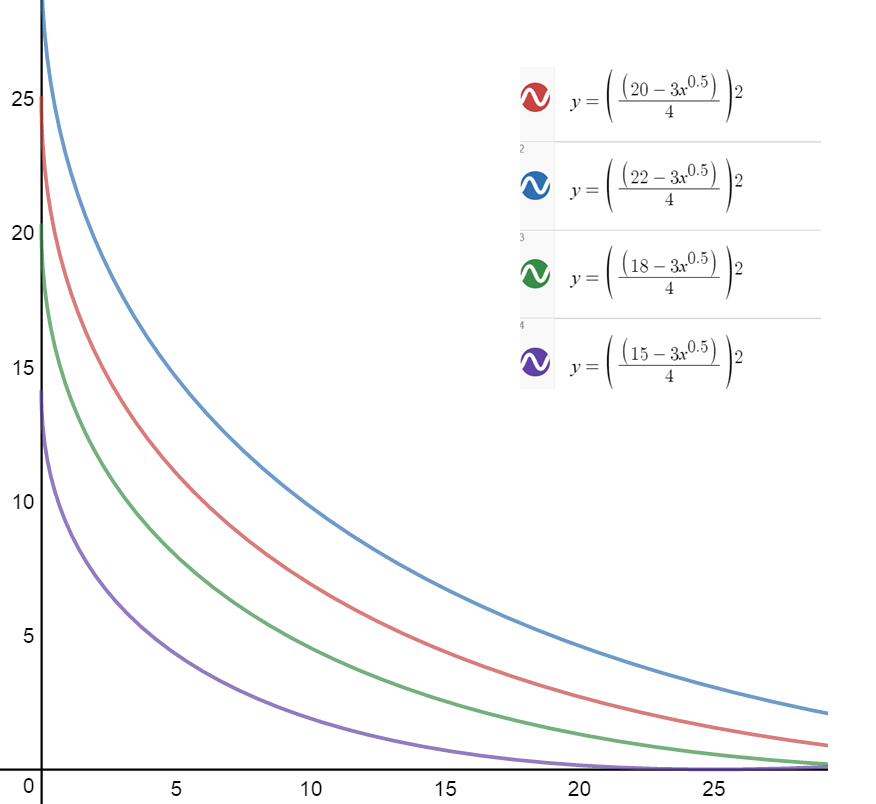
\includegraphics[width=13cm]{Untitled.png}
\end{center}
